\documentclass[11pt,a4paper,twocolumn]{article}
\usepackage[a4paper,top=16.2mm,bottom=16.5mm,left=17mm,right=17mm,columnsep=6.5mm]{geometry}
\usepackage[T1]{fontenc}
\usepackage[utf8]{inputenc}
\usepackage{libertinus}
\usepackage[scaled=.94]{sourcesanspro}
\usepackage{microtype}
\usepackage{graphicx}
\usepackage{amsmath,amssymb,booktabs,tabularx,array,multirow}
\usepackage{xcolor}
\usepackage{hyperref}
\usepackage[backend=biber,style=ieee,sorting=none,maxbibnames=3,minbibnames=1,doi=false,isbn=false,url=true]{biblatex}
\addbibresource{references.bib}
\AtBeginBibliography{\fontsize{8}{9.2}\selectfont}
\usepackage{titlesec}
\usepackage{fancyhdr}
\usepackage{enumitem}
\usepackage{tikz}
\usetikzlibrary{arrows.meta,positioning,shapes.geometric}
\definecolor{navy}{HTML}{17324D}
\definecolor{teal}{HTML}{008E82}
\definecolor{blue}{HTML}{3974A3}
\definecolor{rust}{HTML}{D8754C}
\definecolor{muted}{HTML}{5E7180}
\definecolor{linec}{HTML}{D9E3E9}
\definecolor{paper}{HTML}{F4F7F9}
\hypersetup{colorlinks=true,urlcolor=black,linkcolor=black,citecolor=black,pdftitle={SAE-Gated RAG: Deciding to Answer, Retrieve, or Abstain Before Generation},pdfauthor={Gopal Kataria, Manya Jain, Nidhi Vaidya, Salvik Krishna}}
\setlength{\parindent}{0pt}
\setlength{\parskip}{3.1pt}
\setlength{\columnsep}{6.5mm}
\setlength{\textfloatsep}{9pt plus 2pt minus 2pt}
\setlength{\floatsep}{7pt plus 2pt minus 2pt}
\setlength{\intextsep}{7pt plus 2pt minus 2pt}
\renewcommand{\topfraction}{.94}
\renewcommand{\bottomfraction}{.85}
\renewcommand{\textfraction}{.08}
\renewcommand{\floatpagefraction}{.88}
\setlist[itemize]{leftmargin=1.1em,itemsep=1pt,topsep=2pt,parsep=0pt}
\titleformat{\section}{\sffamily\fontsize{12}{14}\selectfont\bfseries\color{black}}{\thesection.}{.45em}{}
\titlespacing*{\section}{0pt}{9pt}{3pt}
\titleformat{\subsection}{\sffamily\fontsize{10.1}{11.8}\selectfont\bfseries\color{black}}{\thesubsection}{.45em}{}
\titlespacing*{\subsection}{0pt}{6pt}{2pt}

\pagestyle{fancy}\fancyhf{}\renewcommand{\headrulewidth}{0pt}
\fancyfoot[L]{\sffamily\fontsize{7}{8}\selectfont\color{muted} LMA GROUP PROJECT  /  FINAL REPORT}
\fancyfoot[R]{\sffamily\fontsize{7}{8}\selectfont\color{muted}\thepage}
\newcommand{\captext}[1]{\textbf{\color{black}#1}}
\newcommand{\smallnote}[1]{{\fontsize{8.2}{9.3}\selectfont\color{muted}#1}}
\newcommand{\fancyfigure}[3]{\begin{figure}[tbp]\centering\includegraphics[width=\columnwidth]{figures/#1}\caption{#2}\label{#3}\end{figure}}
\makeatletter
\long\def\@makecaption#1#2{\vskip 3pt\small\sffamily\fontsize{7.5}{9.0}\selectfont\color{muted}\noindent\textbf{\color{black}#1.} #2\par}
\makeatother
\begin{document}
\twocolumn[{
\begin{center}
{\sffamily\fontsize{9.0}{10.8}\selectfont\bfseries\color{black}LMA GROUP PROJECT REPORT}\par\vspace{6pt}
\noindent\resizebox{0.985\textwidth}{!}{\sffamily\bfseries\color{black}SAE-Gated RAG: Deciding to Answer, Retrieve, or Abstain Before Generation}\par\vspace{8pt}
{\sffamily\fontsize{9}{10.5}\selectfont\bfseries\color{black}Gopal Kataria$^{1}$ \quad Manya Jain$^{2}$ \quad Nidhi Vaidya$^{3}$ \quad Salvik Krishna$^{4}$}\par\vspace{2pt}
{\sffamily\fontsize{7.7}{9.5}\selectfont\color{black}$^{1}$2023112006 \quad $^{2}$2024102068 \quad $^{3}$2023114005 \quad $^{4}$2023113015}\par\vspace{4pt}
{\sffamily\fontsize{8.2}{10}\selectfont\bfseries\color{black}Link to the repository:}\par\vspace{1pt}
{\sffamily\fontsize{8.3}{10}\selectfont\color{black}\href{https://github.com/bropal404/lma-sae-rag-proj/tree/final-evaluation}{github.com/bropal404/lma-sae-rag-proj/tree/final-evaluation}}\par
\end{center}\vspace{4pt}
}]

\section*{Abstract}
Retrieval-augmented generation (RAG) usually searches before answering, even when a language model already knows the answer or retrieval cannot help. We study a \emph{pre-generation, three-way} controller that chooses \textsc{Answer}, \textsc{Retrieve}, or \textsc{Abstain} from a frozen Gemma 3 4B model's question-only activation. A sparse autoencoder (SAE) probe is compared with a dense-activation probe and four routing baselines over 13,500 distinct benchmark questions and a 21.0-million-passage Wikipedia BM25 index. On 4,000 answerable test questions, the validation-selected SAE router cuts retrieval calls by \textbf{50.8\%} relative to always-retrieve while sacrificing only \textbf{0.35 percentage points} of accuracy. A 200-label strict human audit estimates \textbf{7.5\%} label error. However, the SAE underperforms the selected dense probe by 2.38 points in mean test action macro-F1, and its 234.4 ms median composed latency does not beat always-retrieve's 231.3 ms. Abstention reduces wrong answers on simulated retrieval holes, but also reduces coverage. The results show how sparse internal features can support \emph{efficient retrieval decisions and explicit refusal} before any answer is generated.

\section{Introduction}
RAG augments a language model's parametric memory with retrieved passages. This improves coverage of unfamiliar facts, but retrieving on every question incurs cost and can expose an otherwise correct model to irrelevant context. A retrieval trigger issued \emph{during} generation may also pay for decoding before it acts. Our question is narrower: can internal state \emph{before any generated token} predict whether the model should answer directly, use BM25, or decline?

A sparse autoencoder (SAE) transforms a model's dense residual-stream activation into a much larger feature vector in which \emph{only a small subset of coordinates is active} for a given question. Unlike a dense probe, which must classify a mixture of signals in the original activation, a linear classifier on SAE features can potentially use more selective, interpretable indicators of known facts, uncertainty, and evidence needs (Fig.~\ref{fig:arch}). Sparsity may help disentangle useful signals and inspect decisions, although the encoding also adds computation and need not improve accuracy. We therefore compare SAE and dense probes on the \emph{same frozen model} and measure QA accuracy, retrieval cost, action macro-F1, label quality, unsafe outputs, and latency.

\begin{figure*}[!t]
\centering
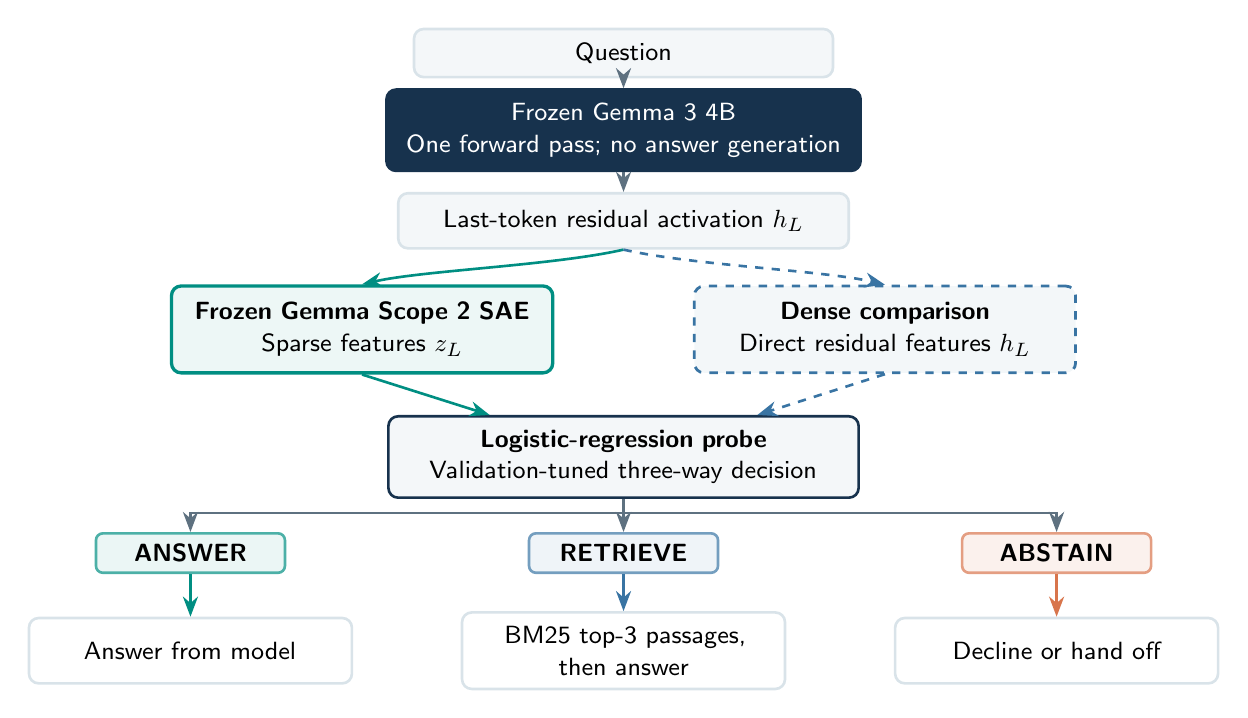
\begin{tikzpicture}[
  >=Stealth,
  line width=.95pt,
  every node/.style={font=\sffamily\fontsize{9.3}{11.4}\selectfont},
  stage/.style={draw=linec,fill=paper,rounded corners=3.5pt,
    text width=4.9cm,minimum height=.56cm,align=center,inner xsep=6pt,inner ysep=5pt},
  model/.style={draw=navy,fill=navy,text=white,rounded corners=3.5pt,
    text width=5.6cm,minimum height=.83cm,align=center,inner xsep=6pt,inner ysep=5pt},
  activation/.style={draw=linec,fill=paper,rounded corners=3.5pt,
    text width=5.3cm,minimum height=.70cm,align=center,inner xsep=6pt,inner ysep=5pt},
  sae/.style={draw=teal,very thick,fill=teal!7,rounded corners=3.5pt,
    text width=4.35cm,minimum height=.97cm,align=center,inner xsep=7pt,inner ysep=6pt},
  comparison/.style={draw=blue,dashed,line width=1pt,fill=blue!6,rounded corners=3.5pt,
    text width=4.35cm,minimum height=.97cm,align=center,inner xsep=7pt,inner ysep=6pt},
  probe/.style={draw=navy,fill=paper,rounded corners=3.5pt,
    text width=5.55cm,minimum height=.77cm,align=center,inner xsep=6pt,inner ysep=5pt},
  labela/.style={draw=teal!70,fill=teal!8,rounded corners=2.5pt,
    font=\sffamily\bfseries\fontsize{9.3}{11}\selectfont,
    minimum width=2.4cm,minimum height=.45cm,align=center,inner sep=4pt},
  labelr/.style={draw=blue!70,fill=blue!8,rounded corners=2.5pt,
    font=\sffamily\bfseries\fontsize{9.3}{11}\selectfont,
    minimum width=2.4cm,minimum height=.45cm,align=center,inner sep=4pt},
  labelx/.style={draw=rust!70,fill=rust!10,rounded corners=2.5pt,
    font=\sffamily\bfseries\fontsize{9.3}{11}\selectfont,
    minimum width=2.4cm,minimum height=.45cm,align=center,inner sep=4pt},
  action/.style={draw=linec,fill=white,rounded corners=3.5pt,
    text width=3.75cm,minimum height=.83cm,align=center,inner xsep=5pt,inner ysep=5pt}
]
% Frozen pre-generation computation.
\node[stage] (q) at (0,0) {Question};
\node[model] (g) at (0,-.98) {Frozen Gemma 3 4B\\One forward pass; no answer generation};
\node[activation] (h) at (0,-2.13) {Last-token residual activation $h_L$};
\draw[->,draw=muted] (q.south)--(g.north);
\draw[->,draw=muted] (g.south)--(h.north);
% The SAE is the proposed path; dense residual features are a comparator.
\node[sae] (s) at (-3.32,-3.51) {\textbf{Frozen Gemma Scope 2 SAE}\\Sparse features $z_L$};
\node[comparison] (d) at (3.32,-3.51) {\textbf{Dense comparison}\\Direct residual features $h_L$};
\draw[->,draw=teal] (h.south) .. controls (-.9,-2.7) and (-2.55,-2.76) .. (s.north);
\draw[->,draw=blue,dashed] (h.south) .. controls (.9,-2.7) and (2.55,-2.76) .. (d.north);
\node[probe] (p) at (0,-5.13) {\textbf{Logistic-regression probe}\\Validation-tuned three-way decision};
\draw[->,draw=teal] (s.south) -- ([xshift=-1.7cm]p.north);
\draw[->,draw=blue,dashed] (d.south) -- ([xshift=1.7cm]p.north);
% Three downstream choices and their actual behavior.
\node[labela] (a) at (-5.50,-6.35) {ANSWER};
\node[labelr] (r) at (0,-6.35) {RETRIEVE};
\node[labelx] (x) at (5.50,-6.35) {ABSTAIN};
\coordinate (fork) at (0,-5.84);
\draw[draw=muted] (p.south)--(fork);
\draw[->,draw=muted] (fork)-| (a.north);
\draw[->,draw=muted] (fork)--(r.north);
\draw[->,draw=muted] (fork)-| (x.north);
\node[action] (aend) at (-5.50,-7.59) {Answer from model};
\node[action] (rend) at (0,-7.59) {BM25 top-3 passages,\\then answer};
\node[action] (xend) at (5.50,-7.59) {Decline or hand off};
\draw[->,draw=teal] (a.south)--(aend.north);
\draw[->,draw=blue] (r.south)--(rend.north);
\draw[->,draw=rust] (x.south)--(xend.north);
\end{tikzpicture}
\caption{Pre-generation three-way routing. The proposed sparse SAE path (teal) and the dense-feature comparator (dashed blue) use separately trained probes. The chosen action answers directly, retrieves BM25 evidence, or abstains.}
\label{fig:arch}
\end{figure*}

\noindent\textbf{Research outcomes.} We test four claims: \textbf{H1} (at least 30\% fewer calls with at most 2 pp accuracy loss), \textbf{H2} (SAE competitive with dense probes), \textbf{H3} (three-way abstention reduces unsafe answers on retrieval holes), and \textbf{H4} (lower median response latency than always-retrieve and verbalised routing).

\section{Literature Review}
\textbf{Adaptive retrieval.} Adaptive-RAG learns retrieval strategy from question complexity \cite{jeong2024adaptive}. Probing-RAG uses intermediate hidden states to decide whether to retrieve \cite{baek2025probing}, the closest conceptual precursor to our two-action comparison. FLARE and DRAGIN instead make retrieval decisions as generation unfolds \cite{jiang2023flare,su2024dragin}; SeaKR uses internal uncertainty to adapt retrieval and reasoning \cite{yao2025seakr}. These approaches motivate the question of when a pre-generation decision can avoid unnecessary steps.

\textbf{Sparse features.} Gemma Scope 2 provides pretrained SAEs for Gemma 3 layers \cite{gemmascope2}; SAE codes offer a feature-space alternative to dense residual activations. We extend hidden-state retrieval probing to an explicit \emph{third action}, and evaluate sparse versus dense choices under the same labels, retrieval system, and budget constraints. This is an empirical comparison, not a claim that SAE-based retrieval decisions are unprecedented.

\section{Dataset Created / Used}
\textbf{Question sets.} We sample 4,000 training, 500 validation and 1,000 test questions each from Natural Questions (NQ) \cite{kwiatkowski2019nq} and TriviaQA \cite{joshi2017trivia}. Generalization tests use PopQA's long-tail entities (1,000, popularity $<100$) \cite{mallen2023pop}, HotpotQA distractor examples (1,000) \cite{yang2018hotpot}, and 500 unanswerable SelfAware questions \cite{selfaware}. A separate 500-item pilot (250 NQ, 250 TriviaQA) is drawn from training data; it is \emph{not} 500 additional independent questions. Seed 13 defines the sampling. The unique question inventory totals \textbf{13,500}; the principal answerable test aggregate covers 4,000 questions, while SelfAware is evaluated separately.

\begin{table}[tbp]\centering\small
\setlength{\tabcolsep}{4.5pt}
\begin{tabular}{@{}lrrrl@{}}\toprule
\textbf{Dataset}&\textbf{Train}&\textbf{Val}&\textbf{Test}&\textbf{Role}\\\midrule
NQ&4,000&500&1,000&Train + test\\
TriviaQA&4,000&500&1,000&Train + test\\
PopQA&--&--&1,000&Long tail\\
HotpotQA&--&--&1,000&Multi-hop\\
SelfAware&--&--&500&Unanswerable\\\bottomrule
\end{tabular}
\caption{Frozen benchmark splits. The 500-question pilot reuses training questions.}\label{tab:data}
\end{table}

\textbf{Retrieval collection.} We build a Pyserini/Lucene BM25 index over \textbf{21,015,324} passages (approximately 100 words each) from the 2018 DPR-style Wikipedia corpus. For each query the retriever scores the top 100 and supplies up to three passages to the generator. We also create \emph{lexical index holes}: on about 30\% of NQ, TriviaQA and HotpotQA questions, top-100 passages with a detected answer alias (or supporting title for HotpotQA) are filtered \emph{at query time}. This tests retrieval failure but does not physically delete documents from the corpus.

\textbf{Gold diagnostic condition.} We choose the highest-ranked top-100 answer-containing passage when available (HotpotQA uses its provided support). These are often \emph{retrieval-derived gold stand-ins}, not independently verified evidence. The same corpus and test split are shared across controllers.

\section{Methodology}
\subsection{Pre-generation three-way gate}
A frozen \textbf{Gemma 3 4B Instruct} model \cite{gemma3} processes only the question (chat template), without decoding an answer. We read the residual-stream vector $h_L\in\mathbb{R}^{2560}$ at the last prompt token of layer $L$; the Hugging Face extraction corresponds to \texttt{hidden\_states[L+1]}. We test $L\in\{9,17,22,29\}$ for both probe families. The sparse path applies a pretrained 16,384-feature, medium-$L_0$ Gemma Scope 2 JumpReLU SAE:
\begin{equation}
 u=W_{\rm enc}h_L+b,\qquad z_j=u_j\,\mathbf{1}[u_j>\theta_j].\label{eq:sae}
\end{equation}
The dense path instead feeds $h_L$ directly to a logistic-regression probe. Neither Gemma nor the SAE is fine-tuned. We train only the class-weighted three-way logistic regression, with \texttt{MaxAbsScaler} for SAE codes and \texttt{StandardScaler} for dense vectors; $C\in\{10^{-3},10^{-2},10^{-1},1,10\}$ is tuned using three-fold cross-validation on macro-F1. A validation-tuned abstention threshold determines the final routed action. Crucially, SAE and dense \emph{layers are selected separately} using NQ/TriviaQA validation, never test performance.



\subsection{Automatic supervision and generation}
Each question is answered under three conditions: \textbf{closed-book}, \textbf{BM25 top-3}, and \textbf{diagnostic gold} where available. We use greedy decoding with at most 32 new tokens; the corrected matcher requires an answer alias as a token span on the first line after SQuAD-style normalization. With $c$ denoting correctness and $u$ an unanswerable case, the \texttt{miss\_as\_retrieve} rule is:
\begin{equation}
 y=\begin{cases}
 \textsc{Abstain}, &u,\\
 \textsc{Answer}, &c_{\rm closed},\\
 \textsc{Retrieve}, &c_{\rm bm25}\lor c_{\rm gold},\\
 \textsc{Abstain}, &\text{otherwise.}
 \end{cases}\label{eq:label}
\end{equation}
The gold-only branch assigns \textsc{Retrieve} to a \emph{retriever miss}, representing the benefit of an improved retriever, not success of the current BM25. The default rule without this branch fails the pilot's label-balance gate.

\section{Experiment Runs}
\textbf{Execution.} Full corpus retrieval (22 Lucene shards) and question splits were validated on the IIIT-H ADA cluster. Gemma generation, SAE extraction, probe grids and latency measurements ran on GPUs (two Tesla T4s for early generation; one NVIDIA L4 for the SageMaker rerun). The final matcher correction fixed 292 previously false-negative answer judgments across closed-book, BM25 and gold outputs before labels and probes were regenerated. Training uses 8,000 NQ+TriviaQA questions; primary tests contain 1,000 each from NQ, TriviaQA, PopQA and HotpotQA, plus the 500-question abstention stress set.

\textbf{Controls and baselines.} \textbf{B1}: always BM25; \textbf{B2}: never BM25; \textbf{B3}: answer-aware oracle (upper bound, not deployable); \textbf{B4}: verbalised generative routing; \textbf{B8}: TF-IDF bigram/unigram logistic regression. A two-way SAE router (no abstention) isolates the effect of the third action. The selected models are \textbf{SAE L29} and \textbf{dense L22}, based on validation macro-F1 of 51.84\% and 53.07\%, respectively. We report classifier macro-F1, routed answer accuracy, retrieval-call rate, abstention/coverage, risk and stage-composed latency; bootstrap comparisons use 2,000 paired, dataset-stratified resamples.

\begin{table}[tbp]\centering\footnotesize\setlength{\tabcolsep}{2.3pt}
\begin{tabular}{@{}lrrl@{}}\toprule
\textbf{Gate}&\textbf{Observed}&\textbf{Requirement}&\textbf{Status}\\\midrule
G0 class minimum&28.0\%&$\geq15\%$&\textcolor{black}{Pass}\\
G1 strict errors&7.5\%&$<10\%$&\textcolor{black}{Point pass}\\
G2 accuracy loss&0.35 pp&$\leq2$ pp&\textcolor{black}{Pass}\\
G2 call reduction&50.8\%&$\geq30\%$&\textcolor{black}{Pass}\\
G3 latency measured&7 methods&Complete&\textcolor{black}{Pass}\\\bottomrule
\end{tabular}
\caption{Gate checks. The G1 upper 95\% confidence limit is 12.0\%, so a population-level $<10\%$ claim is not established.}\label{tab:gates}
\end{table}

\section{Ablations}
\textbf{Layer selection is not monotone.} Validation selects SAE L29 (51.8\%) and dense L22 (53.1\%; Fig.~\ref{fig:layer}). Mean action macro-F1 on the four answerable test sets is instead 45.8\% for SAE L29 and 48.2\% for dense L22. Although SAE L22 attains a higher \emph{test} mean (50.1\%), selecting it after viewing test results would constitute leakage; it is reported only as an explanatory layer ablation.

\fancyfigure{layer_validation.pdf}{Validation-only probe selection. Each dot is macro-F1 averaged over NQ and TriviaQA validation sets; the selections are L29 SAE and L22 dense.}{fig:layer}

\textbf{Feature sparsity and pooling.} At layer 22, exploratory test mean macro-F1 is 50.1\% for standard 16k SAE/L2, 49.6\% for L1, 48.0\% for binarised codes, 46.3\% for 262k-width SAE, and 41.1\% for mean pooling (Fig.~\ref{fig:ablate}). These are supplementary comparisons, not validation-selected changes to the primary router. In the feature-removal diagnostic, zeroing the top 25 class-associated feature groups reduces L22 probe macro-F1 from 53.5\% to 26.2\%; retraining after removal recovers 48.8\%. The effect reflects strong reliance on those coordinates, not proof that their human-interpreted concepts causally determine answers.

\fancyfigure{ablation.pdf}{Exploratory layer-22 SAE variants, full-budget macro-F1 averaged over four test datasets. L1, binarisation, pooling and wider codes change representation and/or probe settings.}{fig:ablate}
\fancyfigure{feature_removal.pdf}{L22 SAE feature removal. Without retraining, masking class-associated coordinates sharply reduces probe F1; retraining recovers part of the loss.}{fig:features}

\textbf{Label budgets.} Both representations improve as supervision grows. At 50 labels, selected SAE/dense mean test macro-F1 are 37.0/40.3\%; at 5,000 they are 45.4/48.4\% (Fig.~\ref{fig:budget}). The initial 1k-to-2k SAE score drop did not reproduce in the later three-seed L17 diagnostic: 53.3\% at 1k, 54.4\% at 2k and 56.3\% at 4k; its original cause remains unresolved.

\fancyfigure{label_budget.pdf}{SAE L29 and dense L22 action macro-F1 versus training-label budget (mean of NQ, TriviaQA, PopQA and HotpotQA test sets; results include three seeds for smaller budgets).}{fig:budget}

\section{Evaluations}
The experiments show a clear trade-off: the SAE-based gate reduces unnecessary searches and can avoid some unsafe answers by abstaining, while a dense probe often predicts the actions more accurately. The benefits are not uniform across datasets, and the SAE route does not deliver a consistent median-latency advantage. We evaluate each claim below against its original criterion.

\subsection{H1: accuracy versus retrieval calls}
The SAE gate achieves \textbf{31.525\%} overall answer accuracy and issues BM25 calls on \textbf{49.175\%} of 4,000 answerable test questions. Always-retrieve scores 31.875\% and calls BM25 100\% of the time. Thus the SAE meets H1's predeclared criterion: \textbf{50.825\% fewer retrievals for only 0.35 pp less accuracy}. Dense L22 achieves 33.975\% accuracy at 60.375\% calls, outperforming SAE in accuracy but retrieving more. TF-IDF makes fewer calls yet sacrifices 4.08 pp versus B1. Figure~\ref{fig:pareto} displays the trade-off; the horizontal dashed line marks the permitted 2 pp degradation from B1.

\fancyfigure{accuracy_retrieval.pdf}{End-to-end accuracy--retrieval trade-off, four answerable test datasets ($n=4{,}000$). The dashed line is 2 pp below always-retrieve; B3 oracle is excluded.}{fig:pareto}

\begin{table}[tbp]\centering\small\setlength{\tabcolsep}{3.8pt}
\begin{tabular}{@{}lrrr@{}}\toprule
\textbf{Router}&\textbf{Answer acc.}&\textbf{BM25 calls}&\textbf{$\Delta$ acc.}\\\midrule
Always retrieve&31.88\%&100.0\%&--\\
Never retrieve&26.38\%&0.0\%&$-$5.50 pp\\
Verbalised B4&31.25\%&64.7\%&$-$0.63 pp\\
TF-IDF B8&27.80\%&38.0\%&$-$4.08 pp\\
\textbf{SAE L29}&\textbf{31.53\%}&\textbf{49.2\%}&\textbf{$-$0.35 pp}\\
Dense L22&33.98\%&60.4\%&$+$2.10 pp\\\bottomrule
\end{tabular}
\caption{Matched routed evaluation on 4,000 answerable questions. Each method uses its validation-tuned decision policy.}\label{tab:routing}
\end{table}

\textbf{Dataset differences matter.} NQ and TriviaQA improve slightly under SAE relative to always-retrieve (+2.3 and +2.0 pp); PopQA drops 5.4 pp and HotpotQA drops 0.3 pp. Dense achieves 34.5\% on PopQA versus SAE's 28.6\%. Thus pooled efficiency gains mask substantial transfer costs (Fig.~\ref{fig:byds}).

\fancyfigure{dataset_accuracy_compact.pdf}{Answer accuracy by dataset (1,000 questions each); the largest SAE weakness is on PopQA.}{fig:byds}

\subsection{H2: sparse versus dense prediction}
The \emph{validation-selected} SAE L29 probe scores 45.8\% action macro-F1 averaged over the four answerable test sets, compared with 48.2\% for dense L22 (\textbf{SAE $-$2.38 pp}), missing the planned 2 pp competitiveness tolerance. These are raw probe-grid results, not routed accuracy. In a separate \emph{validation-threshold routed-action} comparison, SAE is $-$1.91 pp below dense, with a 95\% paired stratified bootstrap confidence interval of \textbf{[$-$3.47, $-$0.28] pp}. Its point estimate is within a 2 pp margin, but the interval crosses the margin; non-inferiority is \emph{not} established. The largest routed macro-F1 deficit is on PopQA ($-$7.68 pp; 95\% CI [$-$10.31, $-$5.00] pp).

\subsection{H3: unsafe answers on index holes}
Across 894 lexical-hole questions (NQ 309; TriviaQA 283; HotpotQA 302), the three-way SAE answers on 84.3\% and makes a wrong answer on \textbf{61.0\% of all hole questions}. Its two-way counterpart always answers and is wrong on \textbf{82.2\%}. The 21.2 pp unconditional reduction comes with lower coverage; conditional error among attempted answers remains 72.3\% for three-way SAE. Figure~\ref{fig:holes} shows both the benefit and the trade-off. The SelfAware slice provides a separate refusal stress test: SAE L29 abstains on 83.2\% of 500 unanswerable questions versus 25.6\% for selected dense L22, but raw answer accuracy is not a meaningful metric for this all-unanswerable slice.

\fancyfigure{hole_risk.pdf}{Simulated lexical holes: the three-way gate reduces wrong answers per \emph{all} hole questions by abstaining more. Coverage is shown to prevent a misleading safety-only comparison.}{fig:holes}

\subsection{Gate 1: supervision quality}
The final pilot labels are \textsc{Answer} 35.4\%, \textsc{Retrieve} 36.6\%, \textsc{Abstain} 28.0\% (Gate 0 passes). After the answer-matcher correction, the strict human audit finds \textbf{15 errors in 200 labels} (7.5\%); its Wilson 95\% interval is 4.6--12.0\%. The alternative, lenient adjudication yields 11\% and does not pass the 10\% point threshold. Results therefore depend on annotation policy, and the strict upper confidence bound does not prove population label error is below 10\%.

\subsection{Gate 3 / H4: response latency}
The final L4 benchmark times the chosen SAE L29 and dense L22 controllers separately at batch size one, using the first 100 test questions from NQ and TriviaQA. It composes controller and generation stage timings with measured BM25 lookup timings; it is \emph{not} a directly timed online serving pipeline. SAE L29 has \textbf{234.4 ms p50}, 466.6 ms p95 and 229.1 ms mean; B1 always-retrieve has \textbf{231.3 ms p50}, 492.8 ms p95 and 273.7 ms mean. SAE therefore \textbf{fails H4's median criterion} (it is 3.1 ms slower than B1), even though its mean is 16.3\% lower and its p95 is 26.2 ms lower. The selected dense probe is 242.6 ms p50; the verbalised router is 427.0 ms p50 (Fig.~\ref{fig:lat}). The SAE controller stage itself has 53.4 ms median cost, versus 52.7 ms for dense.

\fancyfigure{latency_compact.pdf}{Stage-composed latency, fixed 200-question L4 sample. Bars show empirical p50 and p95, not confidence intervals.}{fig:lat}


\section{Limitations}
\begin{itemize}
\item \textbf{Label construct.} Automatic first-line alias matching can miss acceptable paraphrases or accept surface matches without factual entailment. The gold-correct retriever-miss rule targets an improved retriever, not always-realizable BM25 success; strict/lenient audit criteria disagree.
\item \textbf{Synthetic retrieval failures.} Lexical top-100 filtering is not physical index deletion or a natural missing-document distribution. Gold passages may be answer-bearing retrieval stand-ins rather than curated support.
\item \textbf{Representation and transfer.} SAE and dense choose different layers on NQ/TriviaQA validation; their probe families are not perfectly capacity-matched. PopQA transfer degrades under SAE. No fully evaluated dense-retriever shift is claimed.
\item \textbf{Latency scope.} The 200-item timing subset is deterministic, covers only NQ and TriviaQA, and uses composed measured stages. GPU model cache, hardware and retrieval environment are deployment-dependent; improvements in mean/p95 do not imply a median win.
\item \textbf{Statistical scope.} A 7.5\% label-error point estimate has a 12.0\% upper bound; macro-F1 margins and unsafe-answer rates are specific to these sampled benchmark questions and operational definitions.
\end{itemize}

\section{Conclusions}
A pre-generation SAE gate is operationally useful: it saves \textbf{roughly half of BM25 calls} while preserving answer accuracy within the planned two-point tolerance, and it can abstain when retrieved context is misleading or answers are unknown. Nonetheless, the dense probe is stronger in the validation-selected, cross-dataset action comparison; PopQA exposes an important transfer gap; and SAE median latency does not beat always-retrieve on the measured workload. The evidence supports \emph{selective routing with explicit refusal} rather than a universal advantage for sparse representation. Future work should use independently verified evidence, realistic missing-document interventions, broader latency samples and matched-capacity SAE/dense comparisons before drawing stronger deployment claims.

\vspace{-4pt}
\printbibliography[title={References}]
\end{document}
